\documentclass[Arkitektur/System_main.tex]{subfiles}
\begin{document}
\subsubsection{playerSideApp}

\begin{figure}[H]
    \centering
    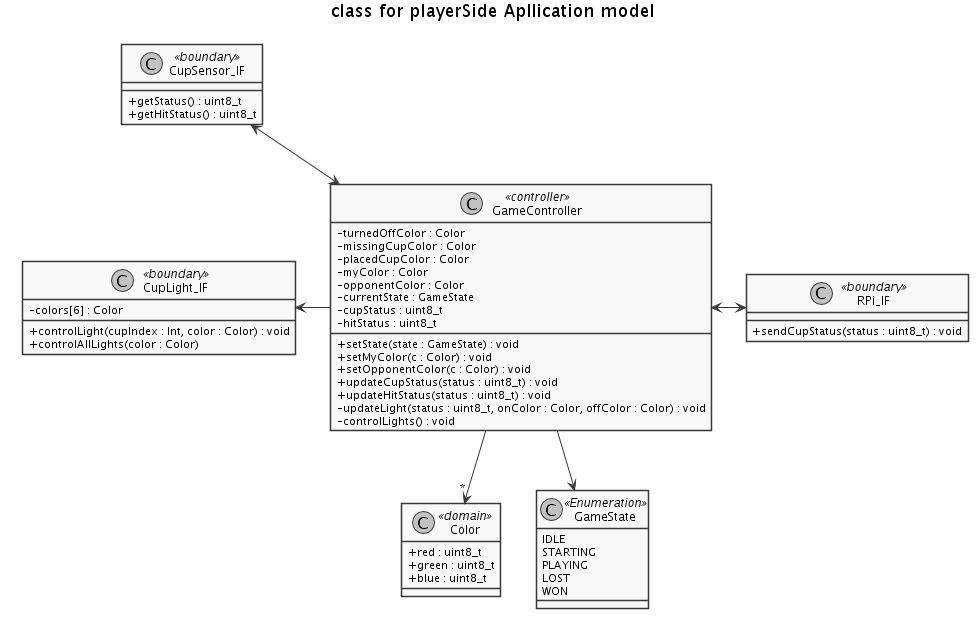
\includegraphics[width=\textwidth]{Arkitektur/Softwarearkitektur/Applikationsmodel/PlayerSide/graphics/classDiagram.png}
    \caption{Klassediagram for playerSideApp}
    \label{fig:CD_PlayerSide}
\end{figure}

\textbf{Controller:  GameController}\\
GameController er den centrale klasse for alle use cases. Den sørger for at sende og modtage data gennem klassen I2C. Alt modtaget data bliver evalueret i GameController og sendt videre i overensstemmelse med protokollen og use case flow. Klassen varetager alt logikken og de flest beslutninger i for player side. 

\textbf{Boundary:  RPi\_IF}\\
Klassen skal modtage kommandoer fra Raspberry pi, og sende data til raspberry pi. Der modtages hovedsageligt data om hvilken tilstand systemet er i og der sendes hovedsageligt koppernes status (om de er der eller ej)

\textbf{Boundary:  CupLight\_IF}\\
Klasse som skal styre lyset under hver kop.

\textbf{Domain:  CupSensor\_IF}\\
Klasse som skal håndtere signal fra Cup sensorerne. Skal informere GameController klassen når der sker en ændring på status på en af kopperne.


\textbf{Domain:  Color}\\
Klasse som bruges til at lagre oplysninger om de forskellige farver der skal bruges.  

\textbf{Enumeration:  GameState}\\
Denne "klasse" er ikke en rigtig klasse. Den bruges til at definere de forskellige tilstande i applicationen. 


\textbf{Tilstandsmaskine for playerSideApp}\\
Programmet byges op omkring en tilstandsmaksine, se figur \ref{fig:playerSide_SM} . Dette er den vigtigste del af denne applikationsmodel. Tilstandene styres af RPi, og afhængig at hvilken tilstand applikationen er i skal der udføres forskellige ting. Der er de fem tilstande: IDLE, STARTING, PLAYING, LOST og WON. IDLE er tilstanden hvor der ikke er nogen der bruger systemet. Her skal der slukkes for alt lys. Dette gøres ved \textbf{entry} for tilstanden. LOST og WON er tilstandene hvor der er fundet en vinder, og den givne side har enten vundet eller tabt. I disse tilstande skal lyset til når man taber eller vinder styres. Når man vinder skal alle kopper lyse med en farve (victoryColor), og når man taber skal de lyse med en anden farve (looserColor). Dette udføres ved \textbf{entry} for tilstandene. STARTING er tilstanden hvor spillet opsættes (svare til UC1). Ved tilstanden STARTING skal lyset under hver kop være styret af om der er en kop eller ej. Hvis der er en kop skal den lyse med en farve og hvis der ikke er en kop skal den lyse med en anden. Dette udføres til dels ved \textbf{entry} for tilstanden. Men det udføres også hver gang Cup sensor detektere en ændring, se sekvensdiagram for tilstand STARTING. Derudover skal der også sendes information om hvilke kopper der er placeret på bordet (status) til RPi når der sker en ændring, men det sendes også ved \textbf{entry}.
PLAYING er tilstanden hvor spillet er i gang (svare til UC2). I tilstanden PLAYING skal der stort set ske det samme som i tilstanden STARTING, det er bare nogle andre farver der skal bruges. 

\begin{figure}[H]
    \centering
    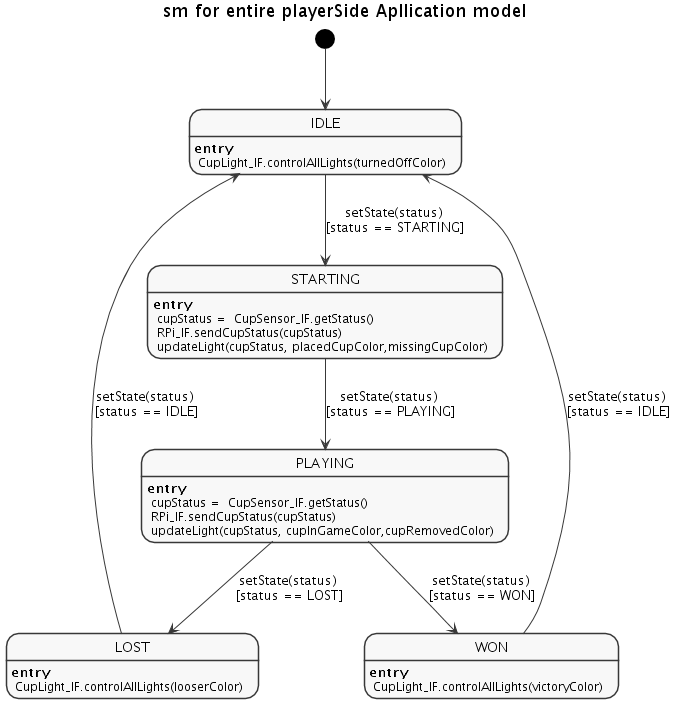
\includegraphics[width=\textwidth]{Arkitektur/Softwarearkitektur/Applikationsmodel/PlayerSide/graphics/state.png}
    \caption{Tilstandmaskine for playerSideApp}
    \label{fig:playerSide_SM}
\end{figure}

\textbf{Sekvensdiagram for STARTING}\\
Der laves sekvensdiagrammer for tilstandene STARTING og PLAYING. Der laves ikke sekvensdiagrammer for de andre tilstande, da der ikke skal ske noget i selve tilstanden, der skal kun ske noget ved \textbf{entry}, og dette er allerede beskrevet i tilstandsmaskinen. Sekvensdiagrammet for STARTING kan ses på figur \ref{fig:playerSide_STARTING_SD}

\begin{figure}[H]
    \centering
    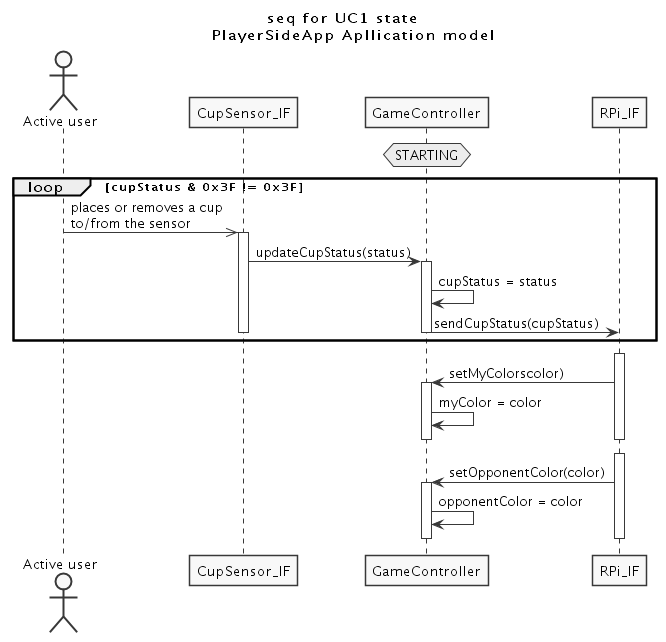
\includegraphics[width=\textwidth]{Arkitektur/Softwarearkitektur/Applikationsmodel/PlayerSide/graphics/UC1_sequence.png}
    \caption{Sekvensdiagram for tilstand STARTING}
    \label{fig:playerSide_STARTING_SD}
\end{figure}
Hver gang der sker tilføjes eller fjernes en kop fra bordet skal denne nye status sendes til GameController og den sørger for at opdatere lysene og sende status til RPi. Der kaldes metoden updateLight som sørger for at indstille hver kop-lys til den angivne farve, afhængig af om der er en kop eller ej. Denne metode er beskrevet i et selvstændigt tilstandsdiagram.

\textbf{Sekvensdiagram for PLAYING}\\
Sekvensdiagrammet for PLAYING kan ses på figur \ref{fig:playerSide_PLAYING_SD}

\begin{figure}[H]
    \centering
    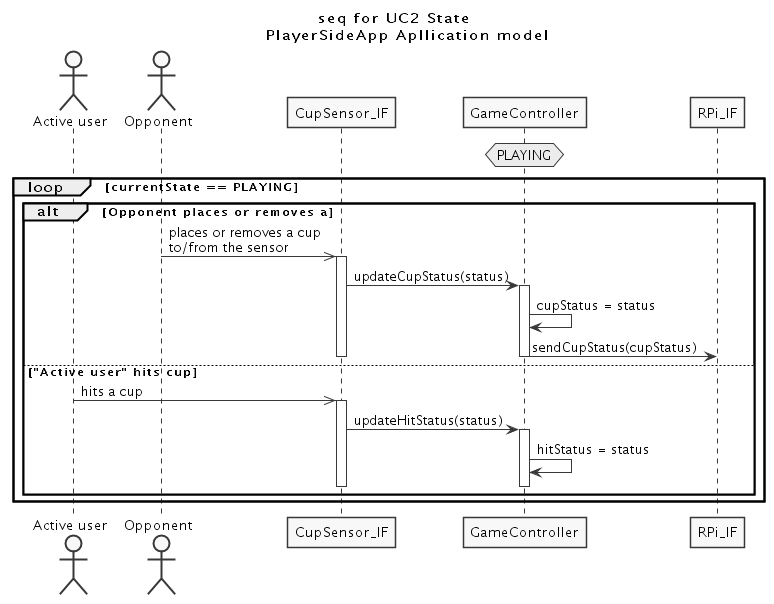
\includegraphics[width=\textwidth]{Arkitektur/Softwarearkitektur/Applikationsmodel/PlayerSide/graphics/UC2_sequence.png}
    \caption{Sekvensdiagram for tilstand PLAYING}
    \label{fig:playerSide_PLAYING_SD}
\end{figure}
Dette diagram er stort set identisk med det for tilstanden STARTING (figur \ref{fig:playerSide_PLAYING_SD}) Den eneste forskel er de farver der bruges. 

\textbf{Sekvensdiagram for updateLight metoden}\\
Der er lavet en separat sekvensdiagram for updateLight metoden, se figur \ref{fig:playerSide_updateLight_SD}. Denne funktion indstiller lyset for hver kop, afhængig af de angivne parametre. 

\begin{figure}[H]
    \centering
    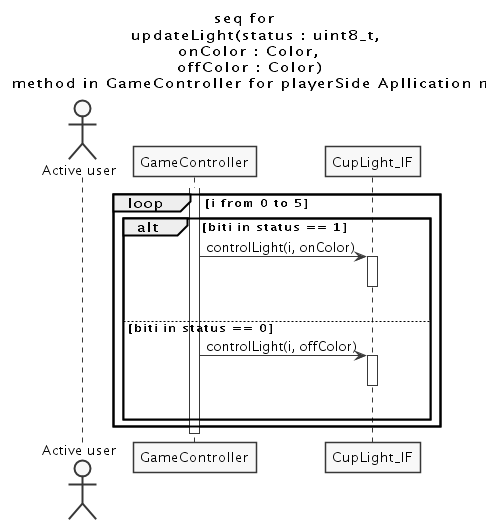
\includegraphics[width=\textwidth]{Arkitektur/Softwarearkitektur/Applikationsmodel/PlayerSide/graphics/updateLight_sequence.png}
    \caption{Sekvensdiagram for updateLight}
    \label{fig:playerSide_updateLight_SD}
\end{figure}

\end{document}